\chapter[The Prime Genesis]{The Prime Genesis: Scaffolding, Node 0, and Terminal Decoupling}
\label{chap:prime_genesis}

\epigraph{
    ``You never change things by fighting the existing reality. To change something, build a new model that makes the existing model obsolete.''
}{--- \textit{R. Buckminster Fuller}, \textnormal{Critical Path} \parencite{fuller1981}}

\epigraph{
    ``The state is a condition, a certain relationship between human beings, a mode of human behavior; we destroy it by contracting other relationships, by behaving differently.''
}{--- \textit{Gustav Landauer}, \textnormal{Revolution and Other Writings} \parencite{landauer2010}}

\epigraph{
    ``A convivial society should be designed to allow all its members the most autonomous action by means of tools least controlled by others.''
}{--- \textit{Ivan Illich}, \textnormal{Tools for Conviviality} \parencite{illich1973}}

We arrive, finally, at the edge of the drafting table.

Throughout this volume, we have walked through the seven autonomous chambers of a new civilizational architecture. We have traced the cold physics of the soil in Layer~1, the silent watchful telemetry of Layer~2, the uncompromising thermodynamic bookkeeping of Layer~3, the deterministic orchestration of Layer~4, the human trust rings of Layer~5, the semantic intents of Layer~6, and the protective legal carapace of Layer~7. In Chapter~11, we watched these layers intertwine across twenty-four living scenarios, demonstrating that a Minimum Viable Society is neither an impossible utopian fantasy nor a detached academic model, but an actionable, testable engineering specification.

Yet a blueprint, no matter how rigorous its mathematical invariants or how thorough its threat vectors, remains inert ink upon paper. A civilization cannot be brought into being by compiling a codebase or issuing an abstract manifesto; it must be inhabited by living bodies on physical ground. We stand now at the threshold where simulation ends and history begins.

To cross that threshold, we must confront the final, unavoidable paradox of our historical moment: the paradox of the scaffolding.

% ============================================================================
% SECTION 12.1: THE ARCHITECTURE OF SCAFFOLDING & THE CENTERING ARCH
% ============================================================================
\section{The Architecture of Scaffolding and the Centering Arch}
\label{sec:scaffolding_centering}

We cannot instantiate a fully sovereign, thermodynamically closed Node on Day~1 without relying on the very legacy infrastructure we intend to obsolete.

This truth is anathema to ideological purists. For generations, intentional communities and radical political experiments have foundered upon the rocks of immediate autarky. Believing that any compromise with the dominant economic system is a moral betrayal, nascent settlements have attempted to step off the grid overnight---refusing corporate software, shunning legal incorporation, and rejecting fiat currency before their own gardens could yield a single bushel of grain. The historical results have been tragically uniform: administrative burnout, physical deprivation, interpersonal fracture, or rapid encirclement and eviction by municipal authorities \parencite{kanter1972, christian2003}.

Conversely, reformist gradualism offers only a slower, quieter death. Initiatives that adopt venture capital, traditional non-profit donor regimes, or corporate cloud platforms ``temporarily'' inevitably find themselves reshaped by the instruments they wield. Without an explicit, mathematically enforced architecture of decoupling, the temporary accommodation calcifies into permanent surrender. The revolutionary initiative degenerates into just another lifestyle business or co-working collective, extracting value from its members to service the mortgages on its real estate \parencite{fisher2009}.

The Sovereign Stack resolves this dialectical dilemma through the principle of \textit{Teleological Scaffolding}, embodied in the historical craft of the \textbf{Medieval Centering Arch} (\textit{le cintre}).

When Gothic builders threw soaring stone vaults across the naves of European cathedrals, cut limestone ashlar blocks could not float in midair. To build an arch of pure compression, master carpenters first erected a massive, temporary timber armature beneath the void. For months, and often for years, those heavy, rough-hewn beams carried the crushing deadweight of the rising stone. The timber was clumsy, combustible, and crude compared to the dressed ashlar it supported. Yet without that wooden centering, no stone vault could ever rise against gravity.

Crucially, the master masons never mistook the timber centering for the cathedral. They did not paint the rough beams; they did not worship the scaffolding. Most importantly, they engineered the centering from Day~1 with \textit{release wedges} and sandboxes at its base. When the final keystone was carved, hoisted into the apex of the vault, and hammered into place, the geometry of the entire structure underwent an instantaneous metamorphosis. The stones locked into mutual, immutable compression. The masons stepped forward with sledgehammers and struck out the wooden wedges. The timber frame dropped away. For the first time, the arch stood under its own gravity, needing neither iron nails nor wooden props to endure for centuries.

Legacy infrastructure---GitHub repositories, POSIX kernels, cloud continuous integration pipelines, Social Purpose Corporations, and fiat bank accounts---is our timber centering frame. We do not worship the wood. We do not apologize for standing upon it. But we engineer it from Day~1 with teleological release wedges in place, so that when the keystone of Node~0 is struck, the scaffolding can be dismantled forever.

\subsection{Beyond Technological Solipsism: Deconstructing the Altruism Fallacy}
\label{subsec:altruism_fallacy}

To engineer genuine release wedges, we must first liberate ourselves from the technocratic blindspot that has crippled previous open-source and cypherpunk movements. Bootstrapping is not merely an engineering progression of software repositories; it is a synchronized evolution of human trust, domestic care, and legal defense.

A lethal error of early communal experiments is what we identify as the \textit{Altruism Fallacy}: the naive assumption that an infant settlement can survive by relying upon the ``unquantified, altruistic labor'' of founding volunteers. As Jo Freeman demonstrated in her classic analysis of informal collectives \parencite{freeman1972}, when an organization disavows formal accounting of labor under the banner of structureless egalitarianism, power and responsibility do not disappear. Instead, they become covert, unaccountable, and concentrated in whoever possesses the unearned external wealth, flexible consulting retainers, or neurotypical stamina to labor eighty hours a week without income. 

Furthermore, as Byung-Chul Han observes in \textit{The Burnout Society} \parencite{han2015}, subjects in modern economies internalize exploitation under the guise of self-fulfillment until depressive collapse. In an unmetered collective, the most conscientious and empathetic members---cooks, caregivers, dispute mediators, and physical menders---burn out first, leaving behind a bitter, technocratic rump.

To prevent structural glue failure \parencite{christian2003}, Phase~1 scaffolding must implement the \textbf{Proto-Ledger (The Mutual Sweat and Care Registry)}. While speculative tokens and external fiat metrics are strictly excluded, the Proto-Ledger formally logs hours of manual site work, culinary sustenance, child accompaniment, and software development. Every hour of foundational sweat equity is cryptographically timestamped and preserved, guaranteeing that early sacrifice translates directly into verifiable Reputational Wealth in Layer~5 the moment the node achieves operational ignition.

\subsection{The Dual-Membrane Doctrine}
\label{subsec:dual_membrane}

In navigating the external world, Node~0 adheres strictly to the \textbf{Dual-Membrane Doctrine} established in Chapter~8. We reject the adversarial rhetoric of early cypherpunks. Terms such as ``Trojan Horse,'' ``parasitic,'' and ``sovereign citizen evasion'' are retired from this architecture. If a nascent community attempts to operate in total illegibility, claiming immunity from municipal zoning, labor law, or property taxes, the legacy state does not dissolve. It responds through its established mechanical instruments: stop-work orders, building condemnation red-tags, Fair Labor Standards Act audits, and sheriff tax foreclosure auctions.

Under the Dual-Membrane Doctrine, the settlement maintains two distinct, un-entangled perimeters:
\begin{enumerate}
    \item \textbf{The External Legal Carapace (Layer 7):} A boring, meticulous, substantively compliant legal shell (Unincorporated Nonprofit Associations, Limited Cooperative Associations, Community Land Trusts, and Perpetual Purpose Trusts). It holds legal title, remits municipal property taxes, enforces life-safety building codes, and answers legal process.
    \item \textbf{The Internal Sovereign Core (Layers 1--6):} Behind this compliant shield, the community operates under pure cryptographic, polycentric self-governance: pairwise Decentralized Identifiers (\texttt{did:peer}), BBS+ Zero-Knowledge selective credentials, the Two-Chamber Assembly, and thermodynamic exergy accounting.
\end{enumerate}

The external carapace acts as an ablative heat shield. It absorbs legacy legal friction so the internal commons may develop the cultural and physical muscle required for eventual terminal decoupling.

% ============================================================================
% SECTION 12.2: THE FOUR PHASES OF EVOLUTIONARY BOOTSTRAPPING
% ============================================================================
\section{The Four Phases of Evolutionary Bootstrapping}
\label{sec:bootstrapping_phases}

The transition from legacy dependence to sovereign autarky unfolds across four methodical, synchronized phases. Each phase represents an evolutionary leap across all seven technical layers alongside a corresponding expansion of human social cohesion and legal armor.

\subsection{Phase 1: The Brittle Shadow (The Scaffolding and Seed Hearth)}
\label{subsec:phase1_shadow}

In the embryonic phase, the project is physically distributed and legally submerged within the Legacy Stack. The founding cohort consists of three to six stewards meeting weekly around a domestic dinner table (The Seed Hearth). Physical exergy is unmetered; economic survival is subsidized by members' legacy employment.

\paragraph{Layer 1 (Physical Reality):} Developers work on consumer laptops powered by the municipal grid, communicating over commercial residential internet service providers. Bare-metal hardware abstraction layers (HAL) interact with virtual serial loops (\texttt{socat} PTYs) and synthetic thermal profiles.
\paragraph{Layer 2 (Digital Twin \& Mesh):} Telemetry is strictly synthetic (\texttt{QUALITY\_SIMULATED}). Sensor streams are generated via the Oasis software-in-the-loop (SITL) bridge over the Universal Human-Agent Interface (UHAI) shared-memory ring buffer (\texttt{/dev/shm}). Reticulum packets tunnel over standard TCP/UDP loopback interfaces.
\paragraph{Layer 3 (Thermodynamic Ledger):} State is recorded in local developer append-logs (RocksDB and SQLite) and traditional git repositories. The Proto-Ledger logs sweat equity hours into encrypted markdown journals. No exergy credits are minted.
\paragraph{Layer 4 (Orchestrator):} Workflows are drafted in standard BPMN 2.0 XML. Execution is verified via Catch2 unit test harnesses running headless \texttt{col-execd} daemon stubs inside sandboxed Wasmtime instances. Continuous integration runs on centralized cloud virtual machines (GitHub Actions).
\paragraph{Layer 5 (Governance):} Identity and access control rely on centralized legacy cryptographic anchors: developer SSH keys, GPG-signed git commits, and repository \texttt{CODEOWNERS} approval rules.
\paragraph{Layer 6 (Semantic Intent):} Intent authoring is conducted in unstructured natural language across legacy issue trackers, parsed manually by developers into W3C JSON-LD test fixtures.
\paragraph{Layer 7 (Legal Carapace):} To defeat the fatal common-law trap of the \textit{unincorporated general partnership} (UPA \S~306)---wherein informal collaborators face joint and several personal liability for project torts and debts---the founders organize as an \textbf{Unincorporated Nonprofit Association (UNA)} pursuant to the Uniform Unincorporated Nonprofit Association Act (UUNAA \S~6) or affiliate with a recognized 501(c)(3) fiscal sponsor. Inbound contributions are defended via Contributor License Agreements (CLAs) enforcing the GNU Affero General Public License (AGPLv3), the CERN Open Hardware Licence (CERN-OHL-S), and the Defensive Patent License (DPL 1.1). Continuous-integration daemons automatically timestamp commit digests to public prior-art registries under 35 U.S.C. \S~102, permanently barring corporate patent trolls. Altruistic volunteer waivers insulate the project against Fair Labor Standards Act wage claims under \textcite{alamo1985}.
\paragraph{Social Architecture:} The Seed Hearth pools emergency fiat reserves into a ring-fenced Legal Defense Escrow, conducts personal metabolic audits, and establishes the foundational practice of weekly shared meals.

\subsection{Phase 2: The Hybrid Bridge (The Headless Engine and Micro-Trials)}
\label{subsec:phase2_hybrid}

The transition to Phase~2 begins when the core C++20 daemons achieve deterministic stability and physical hardware testbenches come online.

\paragraph{Layer 1 (Physical Reality):} Physical transducers make their debut: RS-485 Modbus RTU energy meters, ESP32-S3 current transducers, and DS18B20 temperature probes wired to breadboards in steward workshops.
\paragraph{Layer 2 (Digital Twin \& Mesh):} The \texttt{col-meshd} daemon goes live. It bridges local Semtech SX1262 LoRa transceivers with legacy IP tunnels over WireGuard. Physical telemetry is tagged \texttt{QUALITY\_UNVALIDATED} and ingested into the local UHAI bus.
\paragraph{Layer 3 (Thermodynamic Ledger):} Introduction of local-first CRDTs. The \texttt{col-storaged} daemon initializes an embedded Automerge/Yrs engine. The ledger runs in shadow mode, computing theoretical exergy balances and shadow carbon footprints alongside legacy fiat budgets.
\paragraph{Layer 4 (Orchestrator):} The \texttt{col-execd} daemon deploys as an autonomous POSIX service on local ARM64 edge devices, running the deterministic 10~Hz tick loop. Legacy webhooks trigger signed BPMN start events. Crucially, Oasis functions strictly as an external 3D SITL shadow simulator (Layer 1b); it is never the headless orchestrator.
\paragraph{Layer 5 (Governance):} Transition from repository permissions to cryptographic Decentralized Identifiers (\texttt{did:peer}). Stewards convene physical Key-Signing Parties, deploying Ed25519 threshold signatures (FROST) and issuing initial BBS+ credentials over hardware security enclaves.
\paragraph{Layer 6 (Semantic Intent):} Operational agreements introduce \textbf{Ricardian Contracts} \parencite{grigg2004}. Operational tickets bind natural-language text directly to machine-readable JSON-LD schemas:
\begin{equation}
\mathrm{Contract\_ID} = \mathrm{SHA256}\left(\mathrm{LegalProse}_{\mathrm{markdown}} \parallel \mathrm{Schema}_{\mathrm{JSON-LD}} \parallel \mathrm{Invariants}_{\mathrm{BPMN}}\right)
\label{eq:ricardian_hash}
\end{equation}
Local quantized language models running on edge NPUs validate semantic compliance prior to commit.
\paragraph{Layer 7 (Legal Carapace):} The project incorporates a commercial legal wrapper: a member-governed worker and consumer \textbf{Limited Cooperative Association (LCA)} or \textbf{Social Purpose Corporation (SPC)} with a non-profit indivisible asset lock. The entity publishes the Oasis simulator as an educational game. Under \textcite{howey1946} and \textcite{reves1990}, software sales constitute ordinary consumer transactions. Reputational Wealth carries strictly zero pecuniary properties: no dividends, no equity claims, and continuous thermodynamic decay. The cooperative complies with corporate income taxes, digital sales tax (*South Dakota v. Wayfair*), and W-2 payroll withholding (IRC \S~3402) for full-time core maintainers. Net surplus accumulates in an indivisible reserve for land acquisition.
\paragraph{Social Architecture:} Cohorts engage in georeferenced Oasis rehearsals, run simulated crisis drills (ScDD), conduct 48-hour physical work encampments, and establish Restorative Justice circles.

\subsection{Phase 3: The Sovereign Interface (Physical Inhabitation and Assembly Ignition)}
\label{subsec:phase3_interface}

Phase~3 marks the physical grounding of The Collective. The simulation has completed its rehearsals; the stewards take tools to earth and inhabit physical land.

\paragraph{Layer 1 (Physical Reality):} Full physical deployment of off-grid lifelines: 100~kW photovoltaic arrays, 200~kWh LiFePO4 battery banks with CAN-bus BMS, rainwater cisterns with ultrasonic level transducers, hydronic heating loops, and motorized shunt-trip breakers.
\paragraph{Layer 2 (Digital Twin \& Mesh):} Elimination of cloud relay servers. The Reticulum Network Stack (RNS) operates over 802.11s Wi-Fi mesh and 915~MHz LoRa packet radio. The digital twin reflects live, verified physical telemetry (\texttt{QUALITY\_VERIFIED}).
\paragraph{Layer 3 (Thermodynamic Ledger):} Proof-of-Thermodynamic-Work (PoTW) is activated. Exergy Credits are minted dynamically by \texttt{col-storaged} when cross-validated telemetry proves useful work ($3.6\,\mathrm{MJ} \equiv 1.0\,\mathrm{kWh}$). Credits undergo continuous physical demurrage. Fiat currency is strictly barred from internal circulation.
\paragraph{Layer 4 (Orchestrator):} Workflows execute natively on-node. Centralized cloud CI/CD is replaced by hermetic, bit-for-bit reproducible Nix builds executing on Node~0 clusters. The 10~Hz engine schedules microgrid load shedding, irrigation pulses, and workshop tool allocations without internet access.
\paragraph{Layer 5 (Governance):} Centralized repositories are completely deprecated. Operational governance is exercised through the in-person Key Ceremony (Scenario Omicron). All seven Trust Rings are active; the Two-Chamber Assembly governs resource allocations; the Protocol of Refusal actively shields non-stewards.
\paragraph{Layer 6 (Semantic Intent):} The local Agora runs entirely on-node. Stewards interact via ruggedized Cadastral Slates over local mesh Wi-Fi. Natural-language intents are parsed locally by edge NPUs into signed W3C JSON-LD intents.
\paragraph{Layer 7 (Legal Carapace):} The settlement deploys the \textbf{Dual-Chassis Model}:
\begin{enumerate}
    \item \textbf{The Community Land Trust (CLT):} Fee-simple absolute title to the land and water rights is vested in an independent, non-profit CLT with an indivisible asset lock, removing the earth from speculative commerce and permanently extinguishing partition-by-sale lawsuits.
    \item \textbf{The Steward Worker Cooperative:} The operating cooperative holds a 99-year Ground Lease from the CLT, owning physical improvements with limited liability.
\end{enumerate}
Zoning is navigated via state Accessory Dwelling Unit (ADU) preemption statutes (e.g., California SB~9/10, Washington HB~1110/1337) and agricultural exemptions. Structural timber designs (Scenario Xi) are stamped by licensed Professional Engineers under IRC Appendix AQ/AR/AS. Master Membership Agreements mandate binding arbitration under the Federal Arbitration Act (9 U.S.C. \S\S~1--16), legally shielding internal restorative agreements (Scenario Psi) from judicial interference.
\paragraph{Social Architecture:} Ratification of the Founding Covenant; physical barn-raisings; establishment of the community kitchen, neighborhood tool library, and unconditional public convivial sanctuary.

\subsection{Phase 4: Terminal Decoupling (The Omega Horizon and Perpetual Purpose Trust)}
\label{subsec:phase4_omega}

Phase~4 realizes the terminal decoupling codified in Scenario Omega (\ref{subsec:scn_omega}): striking the wooden centering wedges and entering perpetual homeostatic autarky.

\paragraph{Thermodynamic Invariant:} The settlement mathematically satisfies the Autarky Sovereignty Index:
\begin{equation}
\mathcal{S}_{\mathrm{autarky}} = \min\left( 
    \frac{\Phi_{\mathrm{generation}}}{\Phi_{\mathrm{load}}}, \, 
    \frac{\mathcal{M}_{\mathrm{yield}}}{\mathcal{M}_{\mathrm{caloric}}}, \, 
    \frac{\mathcal{W}_{\mathrm{catchment}}}{\mathcal{W}_{\mathrm{consumption}}} 
\right) \ge 1.25
\label{eq:autarky_index}
\end{equation}
for twelve consecutive lunar cycles across electrical power, caloric sustenance, and potable water.

\paragraph{Physical Decoupling (Layers 1 \& 2):} Motorized 400A automatic transfer switches throw with an echoing mechanical clunk, physically isolating the settlement from the municipal electrical grid forever. Direct underground single-mode dark fiber lines (OS2 10~Gbps) establish sovereign inter-node peering across the watershed. Reticulum mesh transceivers shift to 100\% air-gapped bioregional operation.
\paragraph{Ledger Purity (Layer 3):} Layer~3 permanently erases all fiat currency symbols, foreign exchange APIs, and market price feeds. The currency standard transitions to the absolute thermodynamic standard:
\begin{equation}
1.0\,\mathrm{Unit} \equiv 3.6\,\mathrm{MJ}\,(1.0\,\mathrm{kWh}\mbox{ net exergy}) \equiv 2.0\,\mathrm{kg}\,\mathrm{CO}_2\mbox{ sequestered}
\label{eq:thermo_unit}
\end{equation}
\paragraph{Daemon Liquidation (Layer 4):} The state engine executes the terminal dissolution sequence: verifies unanimous multi-signature consensus across all Trust Rings $\to$ unlinks legacy webhooks $\to$ transmits formal corporate dissolution filings $\to$ terminates the \texttt{col-adversaryd} daemon forever with \texttt{SIGTERM}.
\paragraph{Governance Federation (Layers 5 \& 6):} The Dissolution Consensus Gate is ratified. Layer~5 ratifies the Bioregional Treaty Protocol, federating with sister nodes. Layer~6 Agora routes inter-node intents over libp2p Gossipsub.
\paragraph{Terminal Legal Carapace (Layer 7):} The Social Purpose Corporation files formal Articles of Dissolution under Title~23B RCW Chapter~14. One hundred percent of the real estate, water rights, and physical machinery are conveyed via statutory warranty deed into an \textbf{Irrevocable Perpetual Purpose Trust (PPT)} (pursuant to RCW 11.98.015 or Wyoming Stat. \S~4-10-503). The Trust Charter legally binds property custody directly to the Sovereign Stack's thermodynamic bylaws and Ostrom commons principles in perpetuity. An irrevocable, self-liquidating municipal property tax escrow endowment is funded, ensuring county ad valorem taxes are permanently paid by a custodial trustee, stripping the state of its sole physical instrument of eviction: the tax foreclosure auction. Layer~7 shrinks to its true minimal residue: holding bare title in trust, maintaining property tax immunity, and answering legal process.

\begin{table}[htbp]
\centering
\small
\setlength{\tabcolsep}{3pt}
\begin{tabular}{|p{0.10\textwidth}|p{0.20\textwidth}|p{0.22\textwidth}|p{0.22\textwidth}|p{0.18\textwidth}|}
\hline
\textbf{Layer} & \textbf{Phase 1: Shadow} & \textbf{Phase 2: Hybrid} & \textbf{Phase 3: Living Mesh} & \textbf{Phase 4: Omega} \\
\hline
\textbf{L7: Legal} & UNA / 501(c)(3) fiscal sponsor; DPL 1.1 IP. & Worker LCA / SPC; non-profit asset lock. & Dual-Chassis: CLT bare title + 99-yr ground lease. & Irrevocable PPT; tax escrow; \texttt{col-adv} dead. \\
\hline
\textbf{L6: Intent} & Plaintext issues; Markdown RFCs. & Hybrid JSON-LD embedded in tickets. & Local Agora UI on Cadastral Slates. & Bioregional treaty routing over Gossipsub. \\
\hline
\textbf{L5: Trust} & GitHub \texttt{CODEOWNERS}; SSH/GPG commits. & \texttt{did:peer} test keys; Key-Signing parties. & 7 Trust Rings; BBS+ ZK credentials; Refusal. & Unanimous Dissolution Gate; Bioregional Pact. \\
\hline
\textbf{L4: Exec} & Corporate GitHub Actions cloud CI/CD. & Local \texttt{col-execd} 10~Hz daemon stubs. & Deterministic local Wasmtime; Nix builds. & 10~Hz BPMN engine; \texttt{SIGTERM} to L7. \\
\hline
\textbf{L3: Ledger} & Proto-Ledger sweat logs; zero tokens. & Shadow exergy logging alongside fiat costs. & Live Exergy Credit minting \& demurrage. & Absolute $3.6\,\mathrm{MJ}$ unit; fiat symbols erased. \\
\hline
\textbf{L2: Mesh} & Synthetic loopback telemetry; mocks. & \texttt{col-meshd} LoRa + WireGuard overlay. & Local 802.11s + LoRa RNS; hardware bus. & 100\% air-gapped; dark fiber direct peering. \\
\hline
\textbf{L1: Ground} & Consumer laptops; commercial grid/WAN. & Workshop testbeds; Modbus energy meters. & Physical parcel; 400A microgrid; cisterns. & Motorized ATS islanding; sovereign fiber. \\
\hline
\end{tabular}
\caption{The Seven Layers across the Four Phases of Evolutionary Bootstrapping.}
\label{tab:bootstrapping_layers}
\end{table}

\subsection{The Technical Decoupling Pipeline Matrix}
\label{subsec:decoupling_pipeline}

To provide actionable engineering clarity, Table~\ref{tab:decoupling_pipeline} maps the methodical decoupling pipeline across six critical infrastructure domains.

\begin{table}[htbp]
\centering
\small
\setlength{\tabcolsep}{3.5pt}
\begin{tabular}{|p{0.18\textwidth}|p{0.24\textwidth}|p{0.26\textwidth}|p{0.24\textwidth}|}
\hline
\textbf{Subsystem} & \textbf{Phase 1: Legacy Scaffold} & \textbf{Phase 2--3: Hybrid Bridge} & \textbf{Phase 4: Terminal Autarky} \\
\hline
\textbf{1. Code Repo} & GitHub (monolithic git) & Radicle P2P mirror + local Gitea over RNS & IPLD content-addressed CAR v2 signed by FROST \\
\hline
\textbf{2. Build / CI} & GitHub Actions (Cloud VMs) & Self-hosted ARM64 runners + ccache daemon & Hermetic, reproducible Nix flakes \\
\hline
\textbf{3. Networking} & Public IPv4 / Cloudflare CDN / TLS CAs & WireGuard VPN overlay over dual-stack WAN & 802.11s Wi-Fi mesh + 915~MHz LoRa RNS \\
\hline
\textbf{4. State / Storage} & AWS S3 / Cloud PostgreSQL & Local SQLite + Yrs CRDT gossip sync & RocksDB append-log + Automerge state roots \\
\hline
\textbf{5. Identity / Auth} & GitHub OAuth / passwords & Hybrid \texttt{did:peer} / Ed25519 on hardware keys & ATECC608A HSM + BBS+ ZK-Credentials \\
\hline
\textbf{6. Legal / Econ} & 501(c)(3) sponsor / USD bank account & Worker Coop (LCA/SPC) + internal exergy shadow & Irrevocable Purpose Trust + Pure $3.6\,\mathrm{MJ}$ PoTW \\
\hline
\end{tabular}
\caption{The Technical Decoupling Pipeline Matrix across Infrastructure Domains.}
\label{tab:decoupling_pipeline}
\end{table}

% ============================================================================
% SECTION 12.3: ENGINEERING AND GOVERNANCE BLUEPRINT FOR NODE 0
% ============================================================================
\section{The Engineering and Governance Blueprint for Node 0}
\label{sec:node0_blueprint}

Node~0 is the foundational physical prototype from which all subsequent nodes replicate. It embodies the full convergence of physical resilience, deterministic computing, and unassailable legal shielding.

\subsection{Hardware Architecture and Bill of Materials}
\label{subsec:hardware_bom}

Node~0 rejects exotic, fragile components in favor of accessible, repairable, and thermodynamically efficient hardware:

\begin{enumerate}
    \item \textbf{The Anchor Compute Cluster:} Three Rockchip RK3588 Octa-Core ARM64 single-board computers (4$\times$ Cortex-A76 @ 2.4~GHz, 4$\times$ Cortex-A55 @ 1.8~GHz) equipped with onboard 6.0 TOPS Neural Processing Units (NPUs). Each node carries 32~GB LPDDR4x RAM and dual 1~TB NVMe SSDs configured in RAID-1 mirror with ZFS and native LUKS2 disk encryption. Housed in a 19-inch 2U passively cooled aluminum chassis with conformal coating against humidity.
    \item \textbf{Hardware Security Module (HSM):} Microchip ATECC608A cryptographic co-processor attached via isolated I2C (\texttt{/dev/i2c-1}), storing private root signing keys and physical entropy seeds. Chassis microswitches connected to GPIO trigger cryptographic memory zeroization (\texttt{mlockall} + flash wipe) in the event of an unauthorized physical enclosure breach.
    \item \textbf{Telemetry \& Fieldbus Gateway (Physical HAL):} Dual Espressif ESP32-S3 microcontrollers running Zephyr RTOS, communicating with the RK3588 host over high-speed optocoupled UART. Dual galvanic-isolated RS-485 Modbus RTU transceivers (MAX14840E) monitor solar inverters and energy meters. Dual SocketCAN controllers (MCP2518FD) interface directly with battery management systems.
    \item \textbf{Radio Transceiver Array:} Semtech SX1262 SPI module tuned to 915~MHz (US ISM) / 868~MHz (EU) with 20~dBm power amplifier and low-noise amplifier, mounted to an external 6~dBi fiberglass omnidirectional antenna. Dual-band Qualcomm Atheros QCA9882 mini-PCIe NICs configured in 802.11s open-mesh mode.
    \item \textbf{Thermodynamic Power Subsystem:} 48V DC native bus powered by a 15~kWh LiFePO4 battery bank (16S 3.2V 280Ah EVE cells) with active balance CAN BMS. A 5.0~kW split-phase pure sine wave hybrid inverter with integrated MPPT charge controller. High-speed motorized Automatic Transfer Switch (ATS) capable of sub-16ms islanding, backed by a 24V 50F supercapacitor buffer on the logic rail to ensure zero brownout interruption during grid disconnection.
\end{enumerate}

\subsection{Local Network Segmentation and Zero-Trust Topology}
\label{subsec:network_segmentation}

To prevent lateral exploitation, Node~0 enforces strict physical and VLAN-level network isolation:
\begin{itemize}
    \item \textbf{VLAN 10 (Fieldbus \& Physical Control):} Strictly air-gapped industrial Ethernet. Interfaces exclusively with the RS-485/CAN gateway, inverter controllers, and telemetry sensors. No routing to higher network segments.
    \item \textbf{VLAN 20 (Reticulum Mesh Backbone):} Encapsulated mesh traffic carrying peer-to-peer Reticulum packets over 802.11s Wi-Fi and directional radio links. All traffic is authenticated and end-to-end encrypted at the transport layer.
    \item \textbf{VLAN 30 (Cadastral Commons LAN):} Local WPA3-Enterprise wireless network for member Cadastral Slates and mobile devices. Grants access strictly to the local Semantic Agora and UHAI endpoints via authenticated TLS client certificates.
    \item \textbf{VLAN 40 (Legacy Proxy DMZ):} The sole network segment with physical connectivity to the legacy Internet router. Sandboxed behind strict nftables firewall rules. Accessible exclusively by the \texttt{col-adversaryd} daemon. Features a physical manual rotary kill-switch that severs the physical TX/RX copper wire pairs.
\end{itemize}

\subsection{The Genesis Key Ceremony}
\label{subsec:genesis_key_ceremony}

The establishment of Node~0 begins not with running code, but with the \textbf{Genesis Key Ceremony} (Scenario Omicron)---a physical cryptographic assembly executed by the founding Stewards:
\begin{enumerate}
    \item \textbf{Air-Gap Assembly:} Founding Stewards assemble in an electromagnetically shielded environment (Faraday enclosure). All cellular phones, commercial wearables, and consumer wireless devices are locked in external signal-blocking lockers.
    \item \textbf{Hardware Entropy Accumulation:} The Node~0 anchor unit boots an audited, minimal operating system from write-protected read-only media. Hardware entropy is harvested from multiple physical phenomena: thermal noise diodes, ATECC608A true random number generators, and ambient radio static captured across the SX1262 receiver.
    \item \textbf{FROST 3-of-5 Threshold Schnorr Generation:} Stewards generate the Node~0 Master Authority key using a 3-of-5 Flexible Round-Optimized Schnorr Threshold (FROST) scheme. Five private polynomial key shares are written to five distinct hardware smartcards distributed among five elected trustees. No single human or device ever possesses the complete master private key. Modifying the Genesis Compact or triggering terminal dissolution mathematically requires three trustees to physically present their tokens and execute the threshold protocol.
    \item \textbf{Seeding the Genesis Compact:} The assembled Stewards author and sign the canonical JSON-LD \texttt{GenesisCompact}: establishing immutable ecological floors (aquifer recharge baselines, solar buffer margins), the unconditional survival baseline, and the initial Web of Trust graph. The document is hashed into the immutable Genesis Content Identifier (CID): \texttt{bafygenesisnode0...}.
    \item \textbf{Secure Enclave Anchoring:} The public master verification key and Genesis CID are immutably written into the ATECC608A secure EEPROM.
\end{enumerate}

\subsection{The Deterministic 7-Daemon Bootstrap Sequence}
\label{subsec:daemon_bootstrap}

Upon power-on, Node~0 executes an ordered initialization sequence managed by \texttt{collective\allowbreak-supervisor}. The sequence enforces Strict Adjacency from physical hardware to the legacy membrane:
\begin{equation}
\mathcal{B}_{\mathrm{daemon}} = \prod_{i=1}^{7} \mathrm{Init}\left(\mathcal{L}_i \,|\, \mathcal{L}_{i-1} \equiv \mathrm{READY}\right)
\label{eq:daemon_bootstrap_invariant}
\end{equation}
where $\mathcal{L}_0 \equiv \mathrm{HARDWARE\_OK}$. No daemon $\mathcal{L}_i$ may open its IPC listener until daemon $\mathcal{L}_{i-1}$ has verified its underlying invariant:
\begin{enumerate}
    \item \textbf{Phase 1 (Layer 1, col-telemetryd):} Connects to \texttt{/dev/ttyUSB0} (RS-485) and \texttt{/dev/can0}. Asserts battery voltage $\ge 48.0\,\mathrm{V}$ and inverter thermal safety. Initializes the \texttt{/dev/shm} UHAI ring buffer and binds \path{/run/collective/ipc/l1.sock}.
    \item \textbf{Phase 2 (Layer 2, col-meshd):} Attaches to the SX1262 LoRa SPI bus and 802.11s mesh interfaces. Starts the Reticulum Network Stack (RNS) reactor and binds \path{/run/collective/ipc/l2.sock}.
    \item \textbf{Phase 3 (Layer 3, col-storaged):} Mounts the Automerge/Yrs CRDT state engine and opens the RocksDB append-log at \texttt{/var/lib/}\allowbreak\texttt{collective/}\allowbreak\texttt{ledger/}. Verifies the Genesis Compact CID against the ATECC608A public key and binds \path{/run/collective/ipc/l3.sock}.
    \item \textbf{Phase 4 (Layer 4, col-execd):} Instantiates the Wasmtime runtime engine with deterministic fuel budgets. Loads approved BPMN 2.0 workflows. Enforces Layer~3 exergy reservation requirements. Starts the 10~Hz deterministic tick loop and binds \path{/run/collective/ipc/l4.sock}.
    \item \textbf{Phase 5 (Layer 5, col-kmsd):} Unlocks the encrypted vault using Steward threshold quorum. Loads the Web of Trust Sparse Merkle Tree (SMT). Initializes the BBS+ Zero-Knowledge credential verifier and binds \path{/run/collective/ipc/l5.sock}.
    \item \textbf{Phase 6 (Layer 6, col-commonsd):} Mounts the Oxigraph embedded RDF Quad Store. Loads JSON-LD ontologies and Agora order books. Opens WebSocket/TLS listeners on VLAN~30 for Cadastral Slates and binds \path{/run/collective/ipc/l6.sock}.
    \item \textbf{Phase 7 (Layer 7, col-adversaryd --- Scaffolding Only):} Binds strictly to VLAN~40 (Legacy WAN). Applies outbound rate-limiting and metadata scrubbers, establishing discrete-event queues for legacy interactions. Binds \path{/run/collective/ipc/l7.sock}.
\end{enumerate}

\subsection{Sovereign Edge Services and the Offline Commons}
\label{subsec:edge_services}

Once booted, Node~0 hosts five sovereign core services accessible to the settlement without external internet connectivity:
\begin{enumerate}
    \item \textbf{The Cadastral Service:} A calm web interface served over local HTTPS/WSS to member Cadastral Slates. Stewards view real-time microgrid reserves, cistern water levels, active community tasks, and deliberative Agora proposals.
    \item \textbf{The Offline Epistemic Commons:} Content-addressed ZIM archives containing full local mirrors of critical human knowledge: Wikipedia, Project Gutenberg, Open Source Ecology blueprints, Appropedia permaculture manuals, and the Emergency Medicine Pharmacopeia.
    \item \textbf{The UHAI Simulation Broker:} High-performance shared-memory IPC broker (\texttt{uhai\_}\allowbreak\texttt{ring\_}\allowbreak\texttt{buffer.hpp}) enabling connected Oasis clients to execute software-in-the-loop stress tests against live telemetry without disrupting operations.
    \item \textbf{Sovereign P2P Code Forge:} An embedded Radicle seed node and git mirror running over Reticulum, allowing community developers to pull, branch, test, and sign software updates locally.
    \item \textbf{Edge NPU Intent Compiler:} A 4-bit quantized language model (Llama-3-8B-Instruct GGUF) executing on the RK3588 NPU, compiling steward natural-language voice recordings into structured W3C JSON-LD intents with zero cloud transmission.
\end{enumerate}

\subsection{Operationalizing Ostrom's Principles and the Tri-Centric Boundary}
\label{subsec:ostrom_tricentric}

To ensure institutional endurance, Node~0 operationalizes Elinor Ostrom's Nobel prize-winning commons governance principles \parencite{ostrom1990}, bridging the gap between legacy jurisprudence and distributed systems (Table~\ref{tab:ostrom_evolution}).

\begin{table}[htbp]
\centering
\small
\setlength{\tabcolsep}{3.5pt}
\begin{tabular}{|p{0.24\textwidth}|p{0.34\textwidth}|p{0.34\textwidth}|}
\hline
\textbf{Ostrom Design Principle} & \textbf{Legacy Scaffolding Wrapper (L7)} & \textbf{Sovereign Stack Protocol (L5/L3)} \\
\hline
\textbf{1. Clearly Defined Boundaries} & CLT deed survey; member rosters. & Pairwise DIDs; BBS+ ZK credentials; Trust Rings. \\
\hline
\textbf{2. Congruence with Local Conditions} & Municipal zoning overlays; agricultural permits. & Layer~3 exergy ledger; real-time ecological floors. \\
\hline
\textbf{3. Collective-Choice Arrangements} & Cooperative bylaws; 1-member-1-vote statutes. & Two-Chamber Assembly: Stewardship \& Commons. \\
\hline
\textbf{4. Monitoring of the Commons} & Statutory audits; environmental compliance logs. & Layer~2 telemetry; tamper-evident acoustic/exergy buses. \\
\hline
\textbf{5. Graduated Sanctions} & Contractual damages; member suspension bylaws. & Restorative circles (Scenario Psi); Basic Needs Firewall. \\
\hline
\textbf{6. Fast Conflict Resolution} & Mandatory binding arbitration under 9 U.S.C. \S\S~1--16. & Neutral mediator discovery; CRDT state merge. \\
\hline
\textbf{7. Rights to Organize Recognized} & Lawful recognition of LCA, CLT, and PPT entities. & Air-gapped cryptographic enclaves; zero PII. \\
\hline
\textbf{8. Nested Enterprises} & Bioregional federation agreements (ICA Principle~6). & Subsidiarity: Guilds $\to$ Node Councils $\to$ Bioregional Pacts. \\
\hline
\end{tabular}
\caption{Operationalizing Ostrom's 8 Design Principles across the Scaffolding-to-Sovereignty spectrum.}
\label{tab:ostrom_evolution}
\end{table}

To balance Ostrom's requirement for clear boundaries with Peter Kropotkin's ethic of radical mutual aid \parencite{kropotkin1902}, Node~0 organizes participation into a \textbf{Tri-Centric Boundary Topology} (Figure~\ref{fig:tricentric-topology}):
\begin{enumerate}
    \item \textbf{Ring 0: The Convivial Public Commons (Unconditional Sanctuary):} Open unconditionally to any human being (neighbors, travelers, refugees). Provides clean drinking water, emergency food, solar device charging, tool repair cafes, and medical triage. Conforms to the Social Immunity doctrine (Chapter~9). Holds zero governance voting weight.
    \item \textbf{Ring 1: The Guild and Apprenticeship Commons (Contributors \& Learners):} Open to active volunteers, remote developers, and workshop participants. Members log hours in the Proto-Ledger, utilize shared machine bays, and participate in community kitchen shifts. Holds advisory voice in Stewardship assemblies.
    \item \textbf{Ring 2: The Covenant Stewards (Node Operators \& Legal Custodians):} Full physical residents who hold cryptographic keys to physical relays, legal land trusts, and treasury escrows. Bound by the Founding Covenant, shared metabolic risk, and routine chore rotas. Holds full dual-chamber voting weight.
\end{enumerate}

\begin{figure}[htbp]
\centering
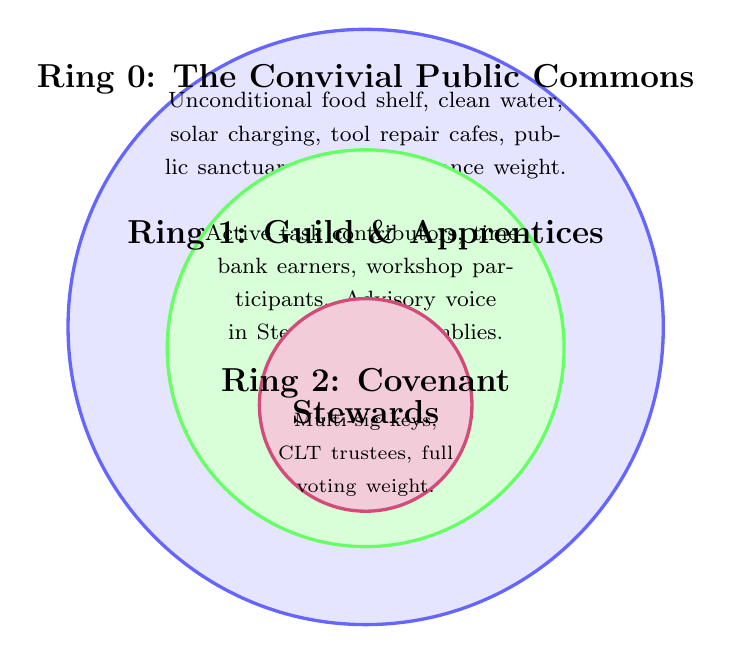
\begin{tikzpicture}[scale=0.9, auto, >=stealth]
    % Outer Ring
    \draw[fill=blue!10, draw=blue!60, very thick] (0,0) circle (4.2cm);
    \node at (0, 3.5) {\textbf{\large Ring 0: The Convivial Public Commons}};
    \node[text width=6.5cm, align=center] at (0, 2.7) {\footnotesize Unconditional food shelf, clean water, solar charging, tool repair cafes, public sanctuary. Zero governance weight.};

    % Middle Ring
    \draw[fill=green!15, draw=green!60, very thick] (0,-0.3) circle (2.8cm);
    \node at (0, 1.3) {\textbf{\large Ring 1: Guild \& Apprentices}};
    \node[text width=4.8cm, align=center] at (0, 0.6) {\footnotesize Active task contributors, timebank earners, workshop participants. Advisory voice in Stewardship assemblies.};

    % Inner Core
    \draw[fill=purple!20, draw=purple!70, very thick] (0,-1.1) circle (1.5cm);
    \node at (0, -0.8) {\textbf{\large Ring 2: Covenant}};
    \node at (0, -1.2) {\textbf{\large Stewards}};
    \node[text width=2.6cm, align=center] at (0, -1.8) {\scriptsize Multi-sig keys, CLT trustees, full voting weight.};
\end{tikzpicture}
\caption{The Tri-Centric Boundary Topology: Reconciling Ostrom's boundaries with radical mutual aid.}
\label{fig:tricentric-topology}
\end{figure}

\subsection{The Founders' Mutual Aid Safety Floor and Institutional Shields}
\label{subsec:safety_floor_shields}


A movement cannot mobilize parents, working-class craftspeople, or marginalized organizers if founding a node requires personal economic martyrdom. Node~0 incorporates four foundational institutional shields:

\paragraph{1. The Founders' Mutual Aid Safety Floor:} The operating cooperative pools incoming revenue from software consulting, fabrication, and agricultural surplus. Before capital is allocated to experimental hardware, it underwrites three safety buffers:
\begin{itemize}
    \item \textbf{Debt and Healthcare Buffer:} Insulating founders from medical precarity and predatory personal debts.
    \item \textbf{Legal Defense Escrow:} Ring-fenced capital with retained counsel to defend stewards against regulatory intimidation.
    \item \textbf{Dignified Exit Guarantee:} In accordance with \textcite{hirschman1970}, any steward retains the unconditional right to leave, guaranteed twelve months of audited severance and relocation support.
\end{itemize}

\paragraph{2. Equipment Stewardship Bailment:} Physical edge servers, batteries, and solar panels are never owned by individual stewards, preventing seizure by personal bankruptcy trustees or judgment creditors. All hardware is held in trust under an irrevocable Equipment Stewardship Bailment Agreement. Custom designs are published under CERN-OHL-S with automated 35 U.S.C. \S~102 prior-art timestamping.

\paragraph{3. Labor Law Defense (*Alamo Foundation* Compliance):} Under \textcite{alamo1985}, providing food and shelter to participants in a commercial business creates an employer-employee relationship under the FLSA. Node~0 strictly bifurcates labor: internal mutual-aid care and permaculture chores are non-commercial acts of the shared domestic household, exempt from the FLSA; commercial export production routes through the cooperative as a statutory Employer of Record, paying lawful wages and issuing compliant W-2s.

\paragraph{4. Local-First Privacy Defense (GDPR Article 4(7) Controller Elimination):} Under the General Data Protection Regulation \parencite{gdpr2016} and the Illinois Biometric Information Privacy Act (BIPA), centralizing personal health or biometric data creates catastrophic liability. Node~0 maintains zero centralized databases of personally identifiable information. Telemetry and credentials remain inside stewards' personal hardware enclaves; verification relies on BBS+ Zero-Knowledge selective disclosure proofs. Legally, Node~0 is not a ``Data Controller'' because it neither determines the means nor the purposes of processing personal data.

% ============================================================================
% SECTION 12.4: THE PROPOSAL AND MANIFESTO FOR NODE 0
% ============================================================================
\section{The Proposal and Manifesto for Node 0}
\label{sec:proposal_manifesto}

This volume does not end with a polite summary. It ends with a summons.

\subsection{The Indictment of the Synthetic Empire}
\label{subsec:indictment}

We do not write for the comfortable spectators of collapse, nor do we seek the applause of academic seminars. We write for those who wake at 2:00~AM in the quiet dark of modern dwellings, gripped by the suffocating realization that the systems sustaining their lives are brittle, fraudulent, and terminally extractive.

You are not crazy for feeling this dread. You are simply paying attention.

The legacy stack of late-stage capitalism is not broken; it is operating with terrifying mechanical efficiency. It was engineered to atomize human communities into isolated consumer households, to sever human hands from the soil, to commodify attention into behavioral surplus \parencite{zuboff2019}, and to liquidate the living biosphere into quarterly dividends for absentee shareholders. It offers frictionless digital conveniences while depleting the water tables beneath our feet. It demands that we spend our creative lifeforces optimizing algorithmic advertisements, while the ecological carrying capacity of our home planet burns around us \parencite{rockstrom2009safe}.

For fifty years, well-meaning movements have marched, petitioned, and occupied. Yet when the tear gas clears, protesters must return to paying rent to legacy landlords, buying poisoned groceries from corporate monopolies, and working for the very megamachine they denounced. Resistance without alternative infrastructure is performative. As Gustav Landauer declared, the state is not an apparatus that can be smashed with a hammer; the state is a social relationship that we destroy by contracting other relationships, by behaving differently toward one another \parencite{landauer2010}.

\subsection{The Affirmation of Ground}
\label{subsec:affirmation_ground}

We refuse to participate in this suicide pact any longer.

Sovereignty is not an ideology; it is a metabolic fact. Technology is not screens; technology is infrastructure for human and ecological life. True wealth is measured not in fiat balances or speculative cryptographic tokens, but in the depth of topsoil, the purity of well water, the stability of microgrids, and the unbreakable trust between neighbors.

Therefore, we announce the founding of \textbf{Node 0}.

Node~0 is not a virtual community. It is not an abstract software repository. It is a physical coordinate on the living earth---a sovereign human settlement where the seven layers of The Sovereign Stack are brought into physical reality simultaneously. It is our reference implementation, our living university, and our sanctuary.

\subsection{The Pioneer Roster across Human Archetypes}
\label{subsec:pioneer_roster}

To build Node~0, we issue our call to five foundational human callings:

\begin{enumerate}
    \item \textbf{To the Silicon Smiths and Systems Architects:} 
    You who understand C++20, bare-metal POSIX daemons, memory-safe runtimes, embedded microcontrollers, and zero-knowledge cryptography. You have spent your careers building platforms that harvest human attention and track human movements. We offer you an honorable trade: leave the surveillance monopolies. Come write the firmware for a nervous system that answers only to the human hands that touch it.
    \item \textbf{To the Soil Stewards and Kinetic Craftsfolk:}
    You who understand the chemistry of thermophilic compost, the geometry of heavy timber framing, the impedance of alternating-current microgrids, the machining of tool steel, and the hydraulics of living watersheds. Without your hands, our code is a ghost wandering through silicon. We need your craft to depave the asphalt, capture the rain, balance the phases, and feed the hearth.
    \item \textbf{To the Caregivers, Mediators, and Social Architects:}
    You who understand the somatic terrain of human trauma, the delicate art of restorative justice, the patience of childcare, and the quiet dignity of elder accompaniment. You are the true keystones of civilization. Communities fail not from external enemies, but from chore resentment and unrecognized emotional labor. We need your wisdom to guide our Welcoming Circles, facilitate our assemblies, and ensure our technology remains a convivial servant of human tenderness.
    \item \textbf{To the Legal Hackers and Structural Strategists:}
    You who understand statutory trusts, municipal zoning exceptions, corporate filings, and property law. We need your intellect to forge our legal armor. Help us structure the Social Purpose Corporations that will shield our early growth; draft the Perpetual Purpose Trusts that will take our land off the speculative market forever; turn the master's own statutes into an impenetrable fortress for the commons.
    \item \textbf{To the Mythmakers, Bards, and Artists:}
    You who write the songs, paint the murals, design the games, and tell the stories that bind human hearts together. A civilization cannot survive on thermodynamics alone. People do not risk their lives for a ledger balance or a network protocol; they risk their lives for beauty, belonging, and love. We need your imagination to bring the Oasis simulation to life, kindle our hearths, and remind us why we endure the struggle to be free.
\end{enumerate}

\subsection{The Constitutional Charter of Node 0}
\label{subsec:constitutional_charter}

\begin{center}
\textbf{\Large THE CONSTITUTIONAL CHARTER OF NODE 0} \\
\textit{Ratified in Physical Assembly by the Founding Stewards}
\end{center}

\vspace{0.5em}
\noindent\textbf{ARTICLE I: THE SOVEREIGN CORE AND BASIC NEEDS FIREWALL.} \\
Node~0 guarantees to every recognized human being within its sanctuary an unconditional, inalienable right to basic physical survival: clean drinking water, caloric sustenance, emergency shelter, and basic healthcare. This survival baseline is an absolute constitutional invariant. It can never be mortgaged, pledged, conditioned upon labor, gated by Reputational Wealth, or revoked as a disciplinary sanction.

\vspace{0.5em}
\noindent\textbf{ARTICLE II: THE INDIVISIBLE COMMONS ASSET LOCK.} \\
The physical soil, watersheds, microgrids, and productive equipment of Node~0 are held in perpetuity for the common good within an Irrevocable Purpose Trust. No individual, trustee, officer, or faction shall ever hold severable equity or private ownership in the commons. The land shall never be divided, partitioned, or mortgaged for speculative gain.

\vspace{0.5em}
\noindent\textbf{ARTICLE III: THERMODYNAMIC BOUNDARIES AND ECOLOGICAL FLOORS.} \\
The economic life of Node~0 is anchored in physical reality. All resource extraction and exergy consumption shall respect inviolable ecological floors. The harvest of living biomass, timber, and water shall never exceed measured biological recharge rates. The currency of internal coordination is the physical exergy of useful work, measured in megajoules, subject to thermodynamic entropy.

\vspace{0.5em}
\noindent\textbf{ARTICLE IV: POLYCENTRIC GOVERNANCE AND THE TWO CHAMBERS.} \\
Governance is exercised through nested, polycentric councils operating under the Two-Chamber standard:
\begin{enumerate}
    \item \textit{The Stewardship Chamber}, weighted by domain-specific Reputational Wealth, decides questions of technical method, engineering execution, and craft competence.
    \item \textit{The Commons Chamber}, operating on the principle of one member, one vote, decides questions of ethical purpose, resource allocation, and communal policy.
\end{enumerate}

\vspace{0.5em}
\noindent\textbf{ARTICLE V: THE PROTOCOL OF REFUSAL AND HUMAN SOVEREIGNTY.} \\
Every Steward retains the inviolable, unpenalized right to invoke the Protocol of Refusal. No algorithmic recommendation, Orchestrator envelope, or council decree may compel a human being to execute an action that violates their conscience, physical safety, or ecological integrity. Sovereign human agency remains the ultimate check on automated systems.

\vspace{0.5em}
\noindent\textbf{ARTICLE VI: PRIVACY BY DESIGN AND CIPHERTEXT INTEGRITY.} \\
The Node recognizes the absolute sanctuary of the human mind and body. Psychological profiles, biometric baselines, and private communications shall remain encrypted inside personal hardware enclaves. The community shall never maintain a centralized registry of intimate data. Verification across councils shall rely exclusively on zero-knowledge proofs.

\vspace{0.5em}
\noindent\textbf{ARTICLE VII: RESTORATIVE JUSTICE AND THE RIGHT OF EXIT.} \\
Disputes between members shall be resolved through facilitated restorative mediation circles seeking reconciliation and restitution. No sanction may withdraw the survival baseline. Every Steward retains the unconditional right to withdraw from the community at any time, carrying their personal records, cryptographic keys, and movable property without penalty or restraint.

\subsection{The Founding Covenant of Node 0}
\label{subsec:founding_covenant}

\begin{quotation}
\centering
\textbf{\large THE FOUNDING COVENANT OF NODE 0} \\[0.3cm]
\textit{Ratified in the presence of the Living Commons and the Assembled Trust Rings.} \\[0.5cm]

\textbf{I. The Pledge of the Indivisible Commons} \\
We declare that this land, this soil, this sunlight, and the tools we assemble are forever liberated from speculative commerce. We hold them not as private masters, but as mortal custodians for the generations unborn. No acre shall be sold; no kilowatt shall be weaponized; no line of code shall be enclosed. \\[0.4cm]

\textbf{II. The Pledge of Radical Conviviality} \\
We reject the coercion of the kinetic state and the invisible violence of the market. We build no weapons; we construct no prisons; we deploy no algorithmic panopticons. Our gates remain open to the hungry, the weary, and the dispossessed. Our mutual defense is rooted in truth, de-escalation, and our indispensability to the bioregional fabric. \\[0.4cm]

\textbf{III. The Pledge of the Shared Floor} \\
We bind our fates together in common risk. While one of us goes cold, none of us is warm. While one of us lacks care, our wealth is an illusion. We pool our burdens, we celebrate our capacities, and we revalue the quiet labor of care with the highest dignity of the Agora. \\[0.4cm]

\textbf{IV. The Pledge of Evolutionary Decoupling} \\
We take the scaffolding of the old world into our hands without shame, but with clear eyes. We will use their tools, their courts, their currencies, and their wire only to weave our own lifelines. And when the thermodynamic loop is closed, we will cut the cord with steady hands, striking down the scaffolding so that the Sovereign Commons may stand alone upon the living earth.
\end{quotation}

\subsection{The 120-Day Tactical Bringup Roadmap}
\label{subsec:roadmap_120days}

The physical manifestations of Node~0 follow a disciplined 120-day bringup sequence across four tactical phases:

\begin{itemize}
    \item \textbf{Days 1--30: The Seed Cohort and Metabolic Baseline (Phase A):} Assemble 6 to 12 founding stewards across the five archetypes. Convene weekly communal hearth dinners; conduct comprehensive metabolic and interpersonal stress audits. Deploy air-gapped Cadastral Slates; initiate private Verifiable Credential mapping. Launch the neighborhood tool library and weekly food-share shelf.
    \item \textbf{Days 31--60: Legal Carapace and Mutual Aid Pooling (Phase B):} File articles of incorporation for the Layer~7 Worker Cooperative / Social Purpose Corporation. Draft the Community Land Trust bylaws with an indivisible asset lock. Capitalize the Founders' Mutual Aid Safety Floor and Legal Defense Escrow. Open wholesale accounts for bulk food staples and photovoltaic equipment.
    \item \textbf{Days 61--90: The Compute Seed and Bioregional Mesh (Phase C):} Procure and configure the 2U air-gapped anchor cluster (RK3588, ATECC608A HSM). Deploy the Reticulum/LoRa packet radio spine across members' dwellings. Ingest regional GIS watershed and soil survey data into the Oasis engine. Rehearse the first six MVS scenarios ($\alpha$ through $\zeta$) in the digital twin.
    \item \textbf{Days 91--120+: Physical Grounding and Genesis Barn-Raising (Phase D):} Acquire fee-simple title to the land parcel through the CLT; execute the 99-year Ground Lease with the operating cooperative. Mobilize the bioregional network for a four-day collective barn-raising: install the 100~kW photovoltaic array, connect the 200~kWh battery bank, erect rainwater filtration cisterns, and commission the commercial kitchen. Flash edge nodes with bare-metal POSIX daemons and connect Modbus transducers. Convene the Genesis Key Ceremony: ratify the Founding Covenant, close the thermodynamic loop, and mint the inaugural Exergy Credit of Node~0.
\end{itemize}

\subsection{The Liturgy of Ignition: Emitting Your Genesis Intent}
\label{subsec:liturgy_ignition}

Do not wait for permission. There is no authority higher than human conscience, and no mandate more urgent than ecological survival.

If you are ready to commit your exergy to the construction of Node~0, you do not begin by waiting for an invitation from on high. You cross the threshold tonight:

\begin{enumerate}
    \item \textbf{Convene the Hearth of Three:} Find two others in your physical geography who carry this same exhaustion and this same resolve. Meet in person. Break bread. Look into each other's eyes and speak the truth of your lives. A sovereign node does not begin with a computer server; it begins with three humans who have resolved never to betray each other to the market.
    \item \textbf{Download the Living Seed:} Clone the project repository. Compile the bare-metal daemons on your local machines. Boot the Oasis engine. Study the twenty-four scenarios. Rehearse the failure modes of human togetherness in simulation before you wager your lives in reality.
    \item \textbf{Stake the Ground:} Map your watershed. Identify the land, the brownfield, or the urban block that can be liberated. Pool your fiat reserves. Form your legal carapace. Take the earth off the speculative market.
    \item \textbf{Emit Your Genesis Intent:} Generate your cryptographic keypair on an air-gapped terminal. Sign the Node~0 Covenant. Emit your \texttt{GenesisIntent} into the mesh. Step into the circle.
\end{enumerate}

Help us build the timber centering. Help us lay the dressed stone. And together, when the keystone is struck, we will take up our hammers, knock out the wedges, and watch the scaffolding fall away into the dust of history.

% ============================================================================
% EPILOGUE CADENCE: STRIKING THE KEYSTONE
% ============================================================================
\section{Epilogue: Striking the Keystone}
\label{sec:striking_keystone}

In the preface to this volume, we began with a confession of exhaustion: the quiet, crushing weariness of living inside a machine that converts living ecology into dead capital. We asked whether it was possible to stop surviving the machine, and start building the garden.

Twelve chapters later, the question is answered.

The garden is not a metaphor. It has a bill of materials. It has a seven-layer architecture. It has twenty-four empirical scenarios. It has cryptographic proofs, thermodynamic bounds, and legal fortifications. It is an engineering reality waiting only for the courage of our hands.

The empire of capital seems all-powerful, omnipresent, and inescapable. But so did the divine right of kings. The legacy stack survives only because we lend it our exergy every morning---because we surrender our labor, our attention, and our children to its gears. The moment we withdraw that exergy, the moment we turn toward our neighbors and pour our sweat into our own soil and our own servers, the spell is broken.

The state is a relationship; we destroy it by contracting other relationships. The machine is a habit; we obsolete it by building the garden.

The C++ compiler is idle, waiting for your commit. The solar panels are unboxed, waiting for your wiring. The compost heap is cold, waiting for your pitchfork. The Welcoming Circle is gathered, leaving an empty chair at the hearth, waiting for you to sit down.

The drafting table is cleared. The blueprint is in your hands.

Build Node~0.
